\section{Gradient Descent}\label{sec:gd}

The process of finding minima or maxima, known collectively as extrema, of a function is not a new endeavor for physicists. After Newton and Leibniz's formulation of calculus we were given analytical procedures for finding extrema by the derivative of functions. From first year calculus we know that a function has an extrema where the derivative is zero, and for many functions and functionals this has a closed form solution. For functionals of complicated functions like neural networks this becomes impractical or impossible. \citet{Mehta2019} also shows that for a simple logistic regression system with $L_1$ regularization the optimization is a transcendental equation requiring iterative methods. Thus we arrive at the hammer which regards any neural network as a nail. Iterative methods of the $n$-th order for finding extrema involves choosing parameters based on the direction of the set of $n$-th order derivatives. In this thesis we will restrict discussions to gradient descent, which is a iterative method of the first order for finding function minima. All the optimization problems are thus cast as minimization problems to fit in this framework. We begin by considering the simplest form of gradient descent of a function of many variables as shown in equation \ref{eq:gd}. 

\begin{equation}\label{eq:gd}
\mathbf{x}_{n+1} = \mathbf{x}_{n} - \eta \nabla f(\mathbf{x}_{n}) 
\end{equation} 

\noindent We known that the gradient vector is in the direction of the steepest ascent for the function, moving towards a minimum then simply requires going exactly the opposite way. The parameter controlling the size of this variable step is  $\eta \in \mathcal{R}_+$. This parameter is dubbed the learning rate in machine learning which is the term we will be using also. The choice of eta is extremely important for the optimization as too low values slow down convergence to a crawl, and can even stall completely with the introduction of value decay to the learning rate. While too large a learning rate jostles the parameter values around in such a way that we might miss the minimum entirely. Figure \ref{fig:badgd} shows the effects of choosing the values for the learning rate poorly, while figure \ref{fig:goodgd} shows the effect of a well chosen eta which finds the minimum in just a few steps. 


\begin{figure}[H]
\centering
\hspace*{-0.9in}
\subfloat[]{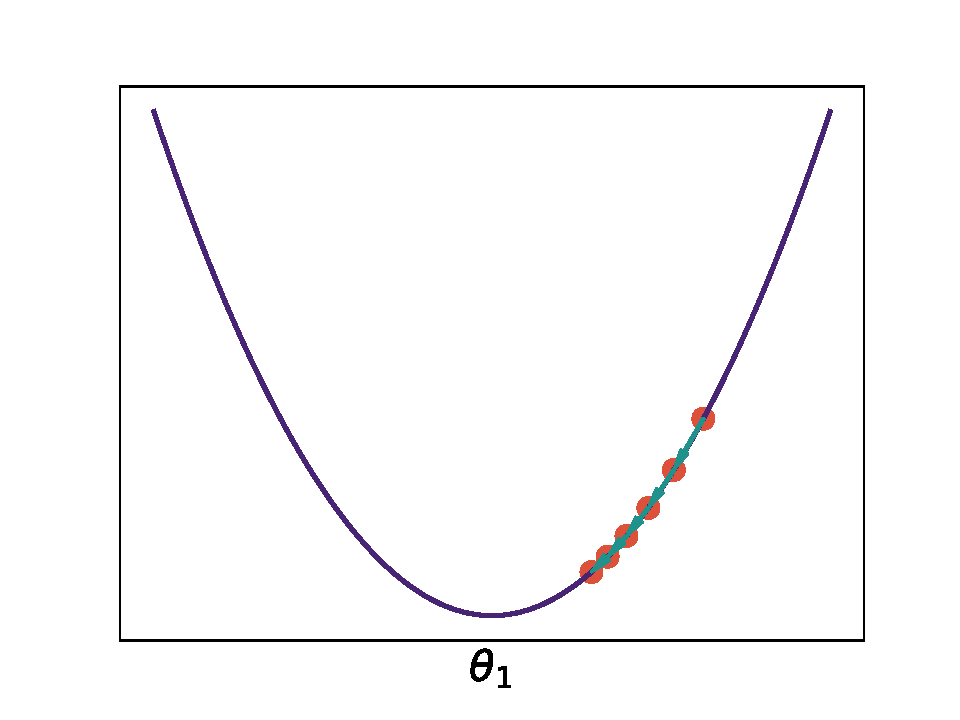
\includegraphics[width=0.6\textwidth]{../figures/gd_low.pdf}}
\subfloat[]{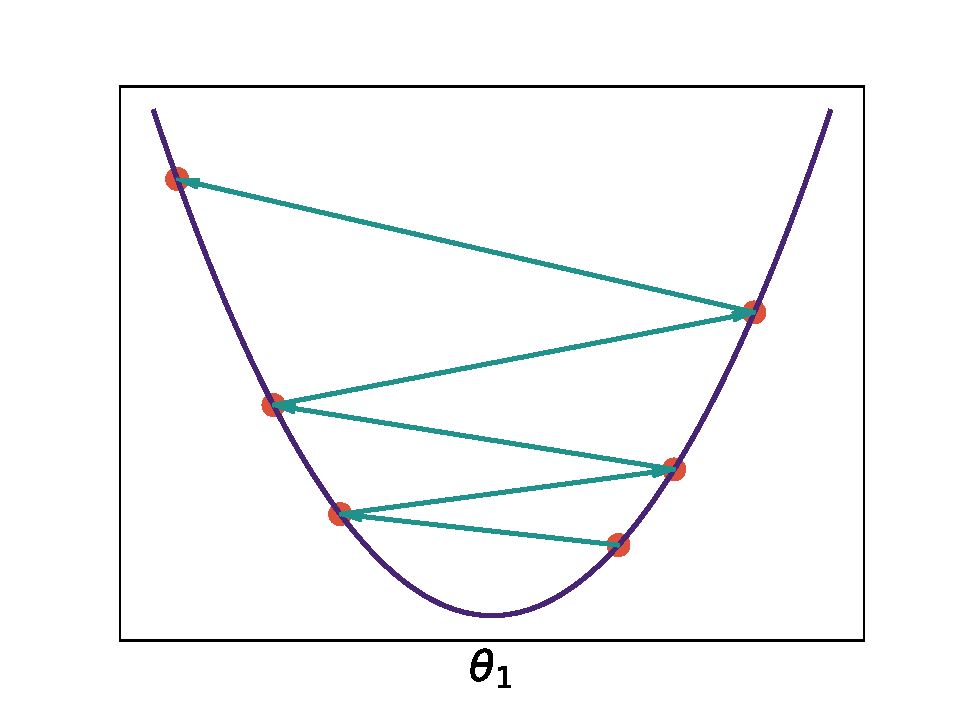
\includegraphics[width=0.6\textwidth]{../figures/gd_large.pdf}}
\caption{Gradient descent on a simple quadratic function showing the effect of too small, \textbf{(a)}, and too large, \textbf{(b)}, value for the learning rate $\eta$}\label{fig:badgd}
\end{figure}

\begin{figure}[H]
\centering
	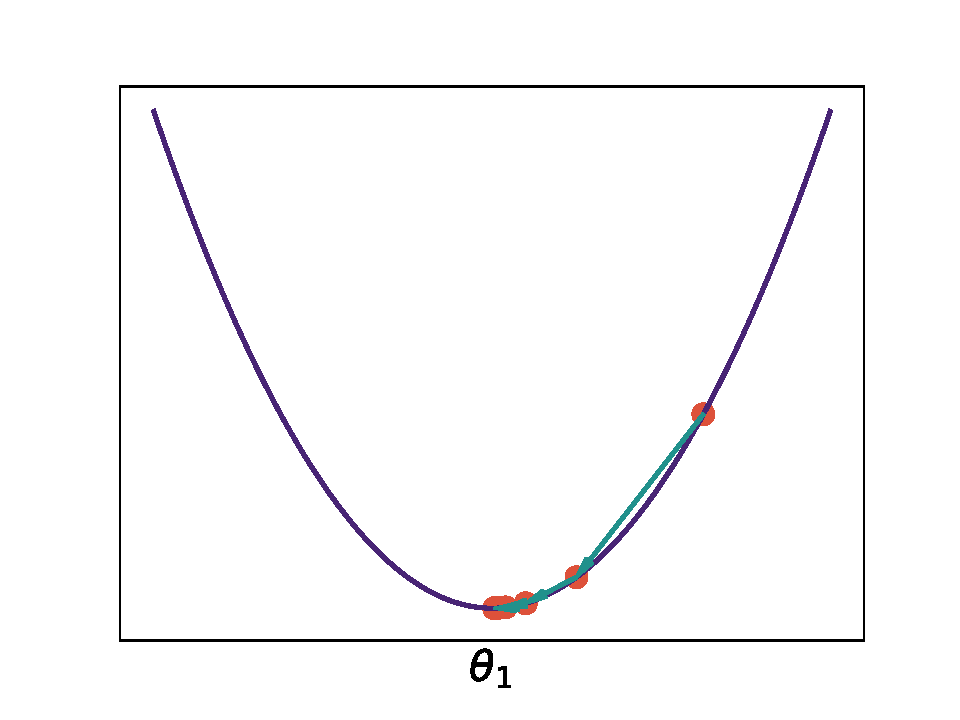
\includegraphics[width=0.75\textwidth]{../figures/gd_good.pdf}
\caption{Complement to figure \ref{fig:badgd} where we show the effect of a good learning rate on a gradient descent procedure. The gradient descent procedure is performed on a quadratic function.}\label{fig:goodgd}
\end{figure}

\noindent While in the case of the convex function we can directly inspect the progress this is not feasible for the high-dimensional updates required for a neural network. In the Stanford course authored by \citet{Karpathy} they point out that one can indirectly observe the impact of the choice of learning rate from the shape of the loss as a function of epoch. This impact is shown in figure \ref{fig:lrloss} which we'll use as a reference when training the models used in this thesis. 

\begin{figure}[H]
\centering
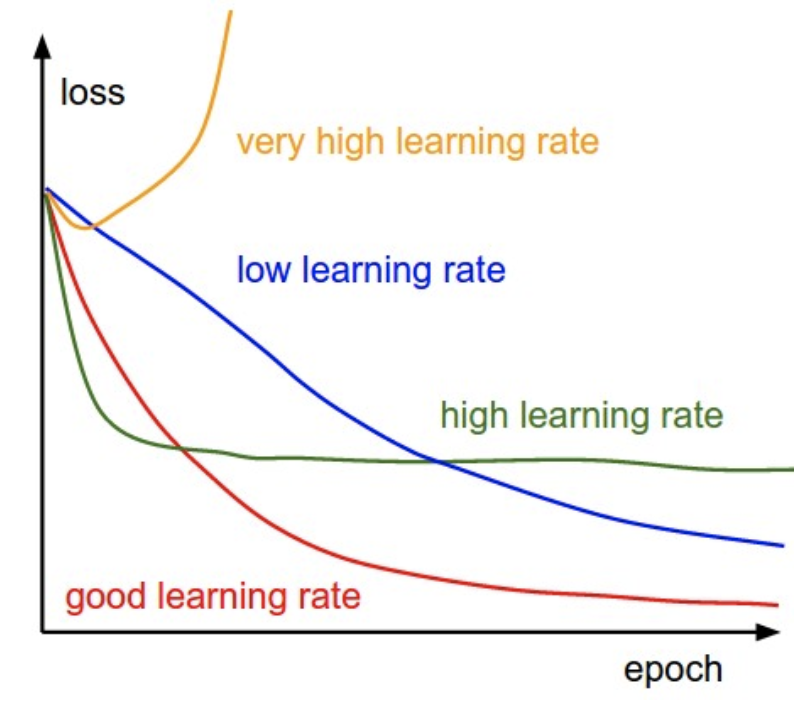
\includegraphics{../figures/lr_loss.png}
\caption{A hand-drawn figure showing the impact of the choice of the learning rate parameter on the shape of the loss function. The optimal choice has a nice slowly decaying shape that we will use as a benchmark when tuning the learning rate in our applications. Copied from the cs231 course material from Stanford authored by \citet{Karpathy}}\label{fig:lrloss}

\end{figure} 

\noindent Using a first order method, while much more computationally efficient than higher order methods, bring with them some problems of their own. In particular there are two problems that need to be solved and we'll go through a couple of methods proposed to remedy them both. 


\begin{enumerate}[start=0, label={(\bfseries C\arabic*):}]
\item Local minima are usually common in the loss function landscape, traversing these while not getting stuck is problematic for ordinary gradient descent
\item Converging to a minima  can be slow or miss entirely depending on the configuration of the method 
\end{enumerate}

The importance of the methods we discuss in the coming sections are also covered in some detail in a paper by \citet{Sutskever2013}. A longer and more in depth overview of the methods themselves can be found in \citet{Ruder}

\subsection{Momentum Gradient Descent}\label{sec:momentum_gd}

The first problem of multiple local minima has a proposed solution that to physicists is intuitive and simple: add momentum. For an object in a gravity potential with kinetic energy to not get stuck in a local minima of the potential it has to have enough momentum, while also not having so much that it overshoots the global minimum entirely. It is with a certain familiarity then that we introduce the momentum update in equation \ref{eq:momentum}

\begin{equation}\label{eq:momentum}
\begin{split}
\mathbf{v}_n &= \beta \mathbf{v}_{n-1} + (1 - \beta) \nabla f(\mathbf{x}_{n}) \\
\mathbf{x}_{n+1} &= \mathbf{x}_n - \eta\mathbf{v}_n 
\end{split}
\end{equation}


\noindent To understand the momentum update we need to decouple the recursive nature of the $\mathbf{v}_t$ term and it's associated parameter $\beta$. This understanding comes from looking at the recursive term for a few iterations

\begin{align*}
\mathbf{v}_n &= \beta(\beta \mathbf{v}_{t-1} + (1-\beta)\nabla f(\mathbf{x}_{n-1})+ (1-\beta)\nabla f(\mathbf{x}_{n}) \\
\mathbf{v}_n &= \beta(\beta (\beta \mathbf{v}_{t-2} \\& \hspace{0.5in}+ (1-\beta)\nabla f(\mathbf{x}_{n-2})) \\& \hspace{0.5in}+ (1-\beta)\nabla f(\mathbf{x}_{n-1})) \\& \hspace{0.5in}+ (1-\beta)\nabla f(\mathbf{x}_{n})
\end{align*}

\noindent So each $\mathbf{v}_t$ is then an exponentially weighted average over all the previous gradients. The factor $1-\beta$ then controls how much of a view there is backwards in the iteration. The factor is then reasonably restricted to avoid overpowering by recent gradients to $\beta \in [0, 1]$. How many steps in the past sequence that this average "sees" we illustrate in figure \ref{fig:beta}. Adding momentum is then a partial answer to the challenge of how to overcome both local minima and saddle regions in the loss function curvature. To summarize we list the parameters that need tuning for a gradient descent with momentum in table \ref{tab:momentum}

\begin{table}
\begin{tabular}{c|c|c|l}
Name &Default value & Scale  & Description\\
\hline
$\beta$  & $0.9$ & Gaussian normal & Exponential decay rate of the momentum step\\
$\eta$  & $10^{-3}$ & Linear & Weight of the momentum update
\end{tabular}
\caption{Hyperparameter table for momentum gradient descent. These parameters have to be tuned without gradient information, we discuss ways to achieve this in section \ref{sec:hyperparams}}\label{tab:momentum}
\end{table}


\begin{figure}
\centering
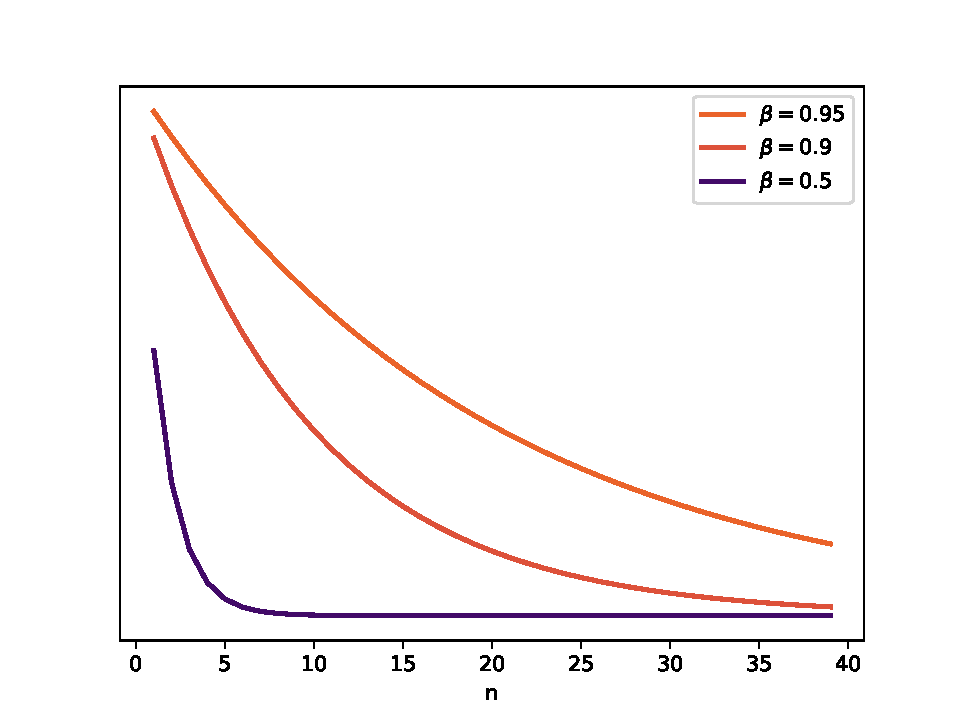
\includegraphics{../figures/beta_decay.pdf}
\caption{A figure illustrating the decay rate of different choices of $\beta$. The lines go as $\beta^n$ and shows that one can quite easily infer how many last steps is included for each choice. A good starting value for the parameter has been empirically found to be $\beta=0.9$ for many applications. In this thesis we'll use a gaussian distribution around this value as a basis for a random search.}\label{fig:beta}
\end{figure}


\subsection{Stochastic \& Batched Gradient Descent}

\subsection{Adaptive Gradient Descent}
\subsection{adam}

